\documentclass[pdf,table]{beamer}
\usepackage{graphicx,hyperref,pdfpages}
\usepackage{tikz}
\usepackage{textpos}
\usepackage{longtable}
\usepackage{listings}
\usepackage{color}
\usepackage{listings}
\usepackage{color}
\usepackage[style=numeric,backend=biber]{biblatex}
%
\usetikzlibrary{arrows}
\usetikzlibrary{positioning,chains,fit,shapes,calc}
\usetikzlibrary{mindmap}
\usetikzlibrary{shapes.multipart}
\usetikzlibrary{decorations.text}
%
\addbibresource{../CST4025.bib}
\setbeamertemplate{bibliography item}{\insertbiblabel}
%
%defin colours
\definecolor{codegreen}{rgb}{0,0.6,0}
\definecolor{codegray}{rgb}{0.5,0.5,0.5}
\definecolor{codepurple}{rgb}{0.58,0,0.82}
\definecolor{backcolour}{rgb}{0.95,0.95,0.92}
\definecolor{delim}{rgb}{20,105,176}



\lstdefinelanguage{CTO}{
	keywords={abstract, asset, by, concept, default, enum, event, identified, Integer, o, participant, String, transaction },
	comment=[l]{//},
	comment=[s]{/*}{*/},
	string=[b]",
	sensitive=true,
}

\lstdefinelanguage{ACL}{
	keywords={transaction,condition,rule,description,participant,operation,resource,action,ALLOW,READ,ALL,CREATE,UPDATE,DELETE,ANY,DENY},
	comment=[l]{//},
	comment=[s]{/*}{*/},
	string=[b]",
	sensitive=true,
}

%define Javascript language
\lstdefinelanguage{JavaScript}{
keywords={typeof, new, true, false, catch, function, return, null, catch, switch, var, if, in, while, do, else, case, break},
keywordstyle=\color{blue}\bfseries,
ndkeywords={class, export, boolean, throw, implements, import, this},
ndkeywordstyle=\color{darkgray}\bfseries,
identifierstyle=\color{black},
sensitive=false,
comment=[l]{//},
morecomment=[s]{/*}{*/},
commentstyle=\color{purple}\ttfamily,
stringstyle=\color{red}\ttfamily,
morestring=[b]',
morestring=[b]"
}
%define json language
\colorlet{punct}{red!60!black}
\definecolor{background}{HTML}{EEEEEE}
\definecolor{delimiter}{RGB}{20,105,176}
\colorlet{numb}{magenta!60!black}

\lstdefinelanguage{json}{
    numbers=left,
    numberstyle=\scriptsize,
    stepnumber=1,
    numbersep=8pt,
    showstringspaces=false,
    breaklines=true,
    frame=lines,
    backgroundcolor=\color{background},
    literate=
     *{0}{{{\color{numb}0}}}{1}
      {1}{{{\color{numb}1}}}{1}
      {2}{{{\color{numb}2}}}{1}
      {3}{{{\color{numb}3}}}{1}
      {4}{{{\color{numb}4}}}{1}
      {5}{{{\color{numb}5}}}{1}
      {6}{{{\color{numb}6}}}{1}
      {7}{{{\color{numb}7}}}{1}
      {8}{{{\color{numb}8}}}{1}
      {9}{{{\color{numb}9}}}{1}
      {:}{{{\color{punct}{:}}}}{1}
      {,}{{{\color{punct}{,}}}}{1}
      {\{}{{{\color{delimiter}{\{}}}}{1}
      {\}}{{{\color{delimiter}{\}}}}}{1}
      {[}{{{\color{delimiter}{[}}}}{1}
      {]}{{{\color{delimiter}{]}}}}{1},
}
%\lstdefinelanguage{json}{
%    numbers=left,
%    numberstyle=\scriptsize,
%    stepnumber=1,
%    numbersep=8pt,
%    showstringspaces=false,
%    breaklines=true,
%    frame=lines,
%    backgroundcolor=\color{backcolour},
%    literate=
%     *{\{}{{{\color{delim}{\{}}}}{1}
%      {\}}{{{\color{delim}{\}}}}}{1}
%      {[}{{{\color{delim}{[}}}}{1}
%      {]}{{{\color{delim}{]}}}}{1},
%}



\lstdefinestyle{mys}{
	backgroundcolor=\color{backcolour},
	commentstyle=\color{codegreen},
	keywordstyle=\color{magenta},
	stringstyle=\color{codepurple},
	numberstyle=\color{codegray},
	basicstyle=\ttfamily\tiny,
	breakatwhitespace=false,
	breaklines=true
	captionpos=b,
	keepspaces=true,
	numbers=left,
	numbersep=5pt,
	showspaces=false,
	showstringspaces=false,
	showtabs=false,
	tabsize=2}
\lstset{style=mys}



\tikzset{every matrix/.style={ampersand replacement=\&,column sep=1.75cm,row sep=2cm},
		BTWMat/.style={ampersand replacement=\&, column sep=0.75cm,row sep=1cm},
		eulerMat/.style={ampersand replacement=\&,column sep=1.1cm,row sep=2cm},
		vertexHighlight/.style={circle,fill=red!80,inner sep=.1cm,text=white},
		vertex/.style={circle,fill=blue!80,inner sep=.1cm,text=white},
		bank/.style={rectangle,fill=blue!50,inner sep=0.1cm,text=black!80}
		edge/.style={--,line width=2pt},
		Dedge/.style={->,line width=2pt},
		DedgeT/.style={->,line width=1pt},
		BiEdge/.style={<->,line width=2pt},
		BiEdgeT/.style={BiEdge,line width=1pt},
		edgeHighlight/.style={--,line width=2pt,color=red},
		loop/.style={min distance=10mm, line width=2pt},
		loopT/.style={min distance=-10mm, line width=1pt},
		label/.style = { rectangle, rounded corners, draw,
		                 minimum width = 2em, fill = yellow!50,
		                 text = red, font = \tiny\bfseries },
		labelT/.style = { circle, draw, line width=1pt,
		                 minimum width = 1em, fill = yellow!50,
		                 text = red, font = \tiny\bfseries },
		every node/.style={align=center}}



\newcommand{\cwideadline}{3$^{rd}$ November 2019}
\newcommand{\cwiideadline}{5$^{th}$ January 2020}
%\newcommand{\cwiiideadline}{31$^{st}$ March 2017}
%\newcommand{\cwiiideadline}{15$^{th}$ April 2018}
\newcommand{\resitdeadline}{1$^{st}$ August 2020}
\newcommand{\deferraldeadline}{1$^{st}$ August 2020}
\newcommand{\deferraldeadlineMay}{1$^{st}$ May 2020}
\newcommand{\moduleCode}{CST4025}
\newcommand{\moduleLeader}{Dr Ian Mitchell }
\newcommand{\theauthor}{Dr Ian Mitchell }
\newcommand{\academicyear}{2019-20}
\newcommand{\email}{i.mitchell@mdx.ac.uk}
\newcommand{\moduleTitle}{Blockchain Development}
\newcommand{\office}{T108}
\newcommand{\officehours}{Autumn \& Winter Terms: Tuesdays 1515-1615hrs; and, Wednesdays 1415-1515hrs}
\newcommand{\tel}{0208-411-6014}
\newcommand{\deptName}{Computer Science}
%\newcommand{\officehours}{Friday 1100\--1300hrs Autumn Term \\ Thursday 1400\--1600hrs Winter Term}
%\newcommand{\officehours}{Autumn Term: Mondays 1300\--1500hrs \\ Winter Term: Thursdays 1400\--1600hrs

\def\bitcoinA{%
  \leavevmode
  \vtop{\offinterlineskip %\bfseries
    \setbox0=\hbox{B}%
    \setbox2=\hbox to\wd0{\hfil\hskip-.03em
    \vrule height .3ex width .15ex\hskip .08em
    \vrule height .3ex width .15ex\hfil}
    \vbox{\copy2\box0}\box2}}



%
\mode<presentation>{
\usetheme{Madrid}
\usecolortheme{beaver}
}
%
\newcommand{\theweek}{10}
\renewcommand{\theequation}{\theweek.\arabic{equation}}

\title[\moduleCode:L\theweek]{\moduleTitle \\ Week: \theweek \\ Title: Case Study} 
\institute[]{\includegraphics[scale=0.25]{../../../logo/mdxSmall} \\ Middlesex University, \\Dept. of Computer Science, \\London}
\author[\textcopyright \email]{\moduleLeader}
\date{\today}




\begin{document}
	\begin{frame}
		\titlepage
	\end{frame}


\addtobeamertemplate{frametitle}{}{%
\begin{textblock*}{100mm}(.94\textwidth,-0.85cm)
\includegraphics[scale=0.1]{../../../logo/transparent}
\end{textblock*}}

	\begin{frame}{Lecture Aims}
		\begin{block}{Aims}
			To gain a holistic view of a blockchain application by investigating the parts, then see how these parts combined add up to more than the whole.
		\end{block}
	\end{frame}

	\begin{frame}{Lecture Objectives}
		\begin{block}{Case Study}
			Today's lecture will investigate the blockchain implementation of evidence management for a forensic lab, colloquially known as a chain-of-custody \cite{mitchell:2019c}
		\end{block}
	\end{frame}


\begin{frame}{Chain of Custody \cite{SWDGE:v3}}
	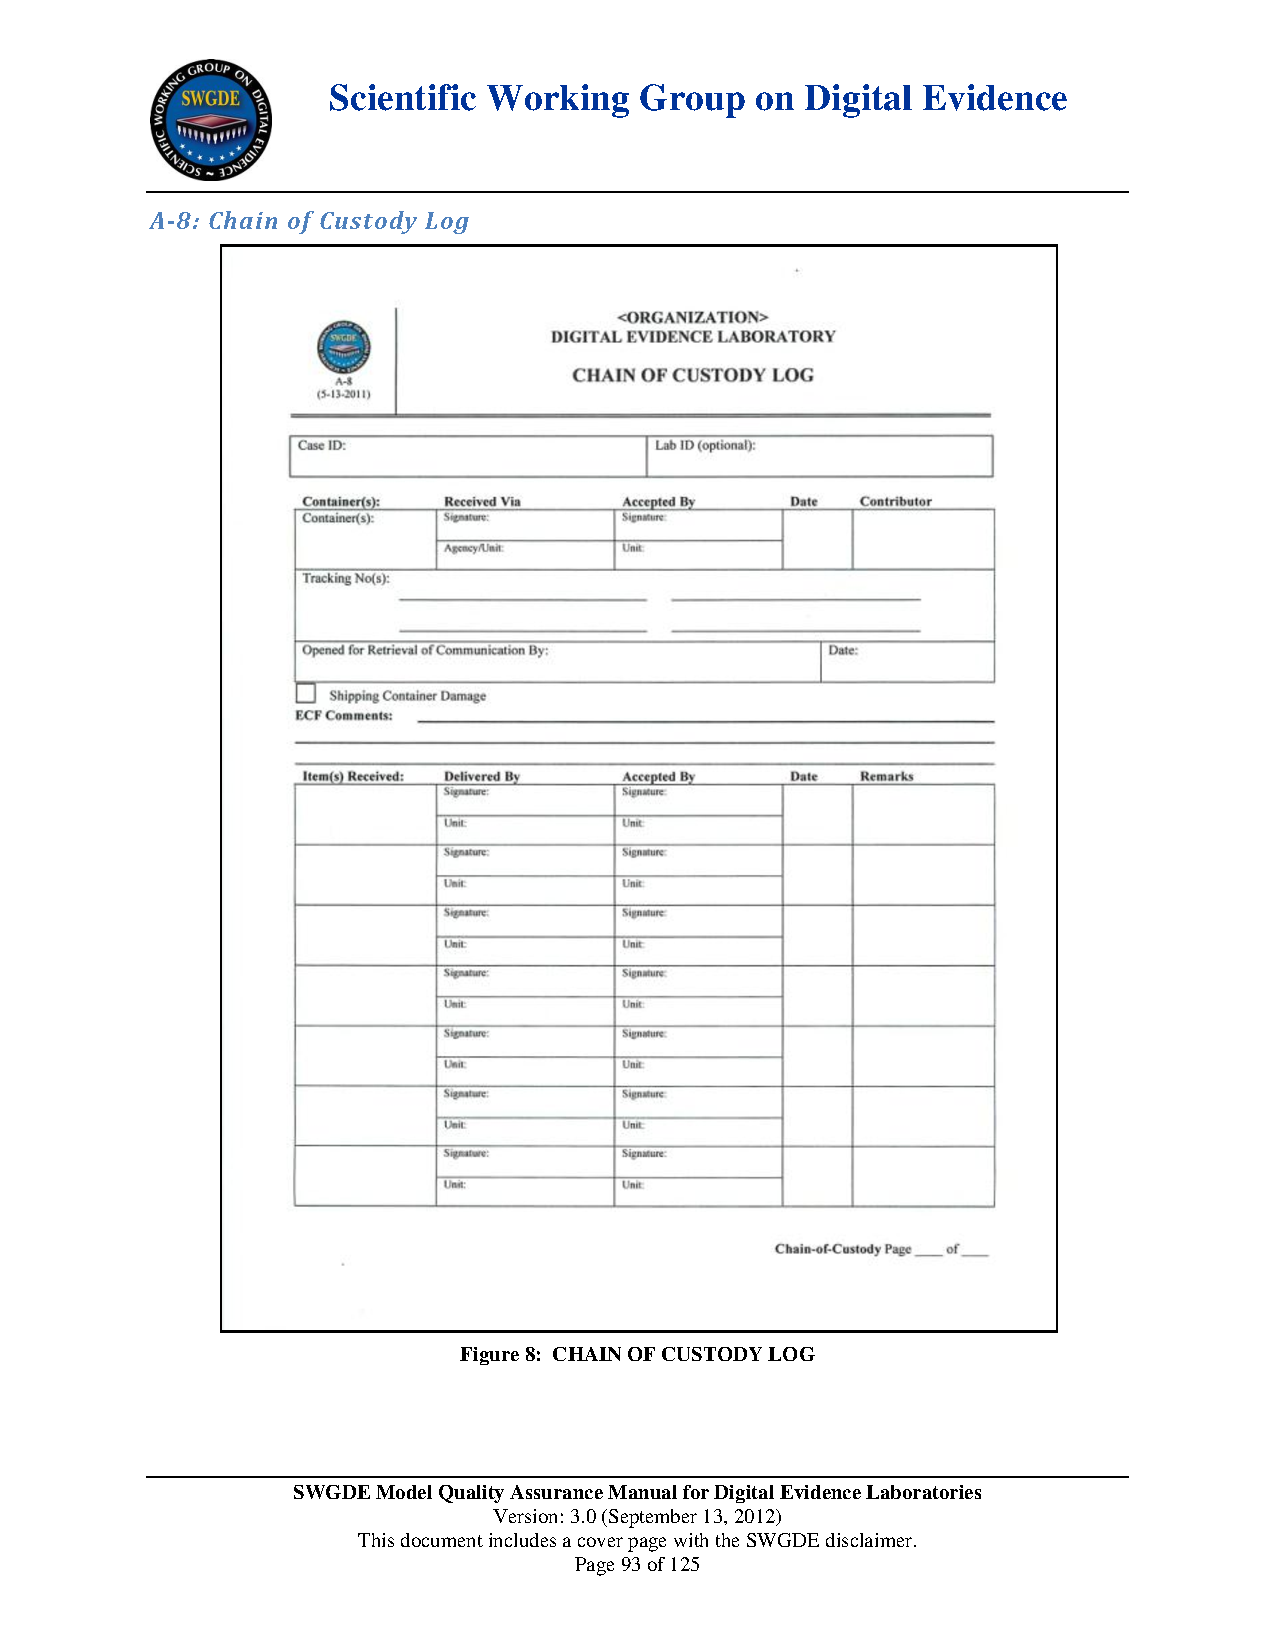
\includegraphics[page=1,width=0.9\textwidth]{coc.pdf}
\end{frame}

\begin{frame}{Chain of Custody \cite{SWDGE:v3} }
	\includegraphics[page=2,width=0.9\textwidth]{coc.pdf}
\end{frame}

\begin{frame}{Chain of Custody\cite{SWDGE:v3}}
	\includegraphics[page=3,width=0.9\textwidth]{coc.pdf}
\end{frame}


\begin{frame}{Use Case Diagram}
	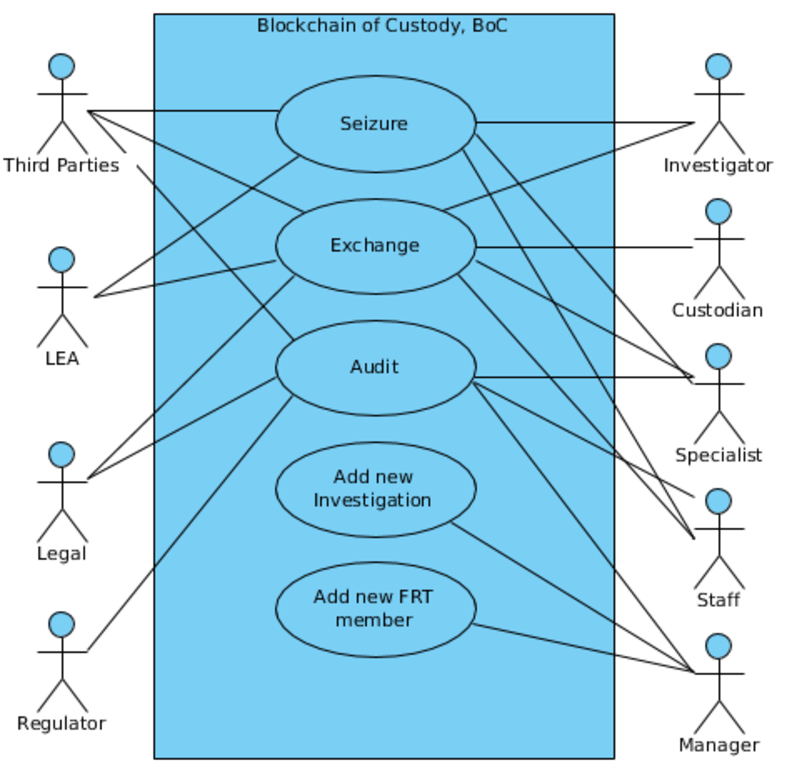
\includegraphics[scale=0.60]{uc6.pdf}
\end{frame}

\begin{frame}{Class Diagram}
	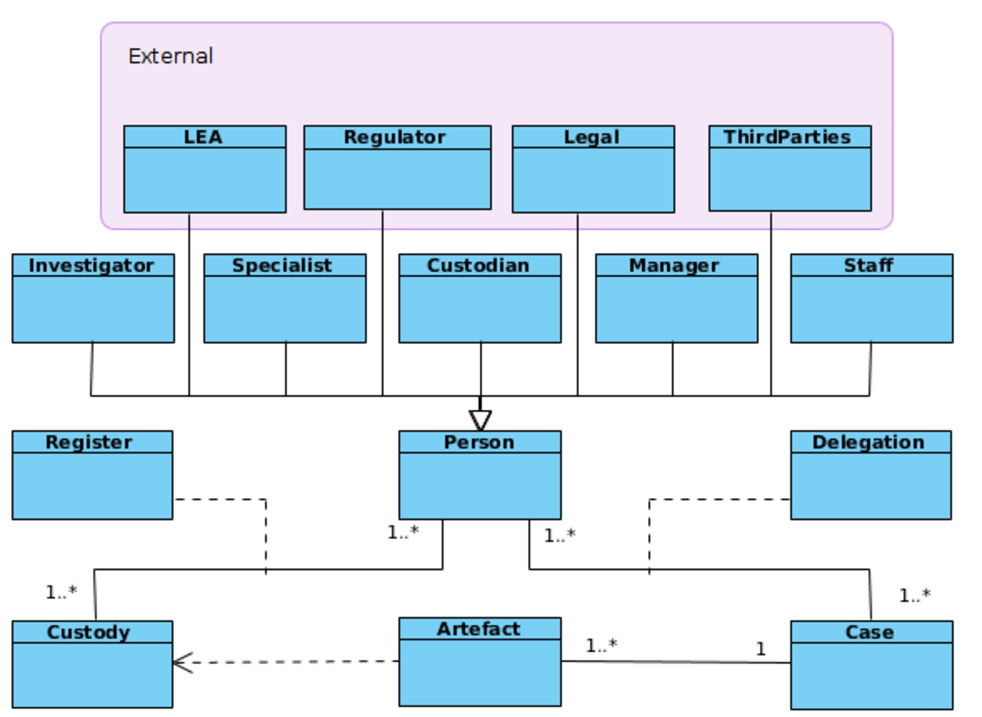
\includegraphics[scale=0.65]{cd6.pdf}
\end{frame}


\begin{frame}[fragile,allowframebreaks]{CTO}{Listing}
	\lstinputlisting[language=CTO]{../boc/models/model.cto}
\end{frame}

\begin{frame}[fragile,allowframebreaks]{ACL}{Listing}
	\lstinputlisting[language=ACL]{../boc/permissions.acl}
\end{frame}


\begin{frame}{Adding a new investigation}
\begin{tikzpicture}
%Add investigation transaction
	\node at (0,7) 		[term] (11){Add New Investigation};
	\node at (0,6)		[proc] (12){Log in};
	\node at (0,4.5)	[test] (13){Manager?};
	\node at (0,3)		[proc] (14){Select Case ID};
	\node at (0,1.5)	[test] (15){Exists?};
	\node at (2,1.5)	[zero] (10){\hfill};
	\node at (2,3)		[proc] (19){Update denied};
	\node at (0,0)		[proc] (18){Update Blockchain};
	\node at (2,6)		[proc] (16){Access \\ Denied};
	\node at (2,0)		[term] (111) {End};
	\node at (2,4.5)	[zero] (17){\hfill};
	\draw[solid,->,>=triangle 60] (11) -- (12);
	\draw[solid,->,>=triangle 60] (12) -- (13);
	\draw[solid,->,>=triangle 60] (13) -- (14);
	\draw[solid,->,>=triangle 60] (14) -- (15);
	\draw[solid]				  (13) -- (17);
	\draw[solid,->,>=triangle 60] (17) -- (16);
	\draw[solid,->,>=triangle 60] (16) -- (12);
	\draw[solid,->,>=triangle 60] (15) -- (18);
	\draw[solid,->,>=triangle 60] (18) -- (111);
	\draw[solid] (15) -- (10);
	\draw[solid,->,>=triangle 60] (10) -- (19);
	\draw[solid,->,>=triangle 60] (19) -- (14);
	\path(13) to node[plainLabel,below]{N} (17);
	\path(13) to node[plainLabel,right]{Y} (14);
	\path(15) to node[plainLabel,below]{Y} (10);
	\path(15) to node[plainLabel,right]{N} (18);

	\node at (3.25,7) 	[zero] 	(100) 	{\hfill};
	\node at (3.25,0)	[zero]	(101)	{\hfill};
	\draw[dashed] (100)--(101);

	\node at (6.5,7)		[term] 	(21)	{Add FRT \\ Member};
	\node at (6.5,6)		[proc]	(22)	{Log in};
	\node at (6.5,4.5)	[test]	(23)	{Manager?};
	\node at (6.5,3)		[proc] 	(24)	{Add Staff};
	\node at (6.5,1.5)	[test]	(25)	{Exist \& Qualified?};
	\node at (9.5,1.5)	[proc]	(26)	{Update Blockchain};
	\node at (4.5,6)		[proc]	(27)	{Access Denied};
	\node at (4.5,4.5)	[zero]	(28)	{\hfill};
	\node at (4.5,1.5)	[zero]	(29)	{\hfill};
	\node at (4.5,3)		[proc]	(211)	{Update denied};
	\node at (9.5,3)		[test]	(212)	{Another?};
	\node at (9.5,4.5)		[term]	(213)	{End};

	\draw[solid,->,>=triangle 60] (21) -- (22);
	\draw[solid,->,>=triangle 60] (22) -- (23);
	\draw[solid,->,>=triangle 60] (23) -- (24);
	\draw[solid,->,>=triangle 60] (24) -- (25);
	\draw[solid] 					(23) -- (28);
	\draw[solid]					(25) -- (29);
	\draw[solid,->,>=triangle 60] (28) -- (27);
	\draw[solid,->,>=triangle 60] (27) -- (22);
	\draw[solid,->,>=triangle 60] (29) -- (211);
	\draw[solid,->,>=triangle 60] (211) -- (24);
	\draw[solid,->,>=triangle 60] (25) -- (26);
	\draw[solid,->,>=triangle 60] (26) -- (212);
	\draw[solid,->,>=triangle 60] (212) -- (213);
	\draw[solid,->,>=triangle 60] (212) -- (24);
	\path(23) to node[plainLabel,below]{Y} (24);
	\path(23) to node[plainLabel,below]{N} (28);
	\path(25) to node[plainLabel,below]{Y} (26);
	\path(25) to node[plainLabel,below]{N} (29);
	\path(212) to node[plainLabel,below]{Y} (24);
	\path(212) to node[plainLabel,right]{N} (213);
\end{tikzpicture}
%\caption{Flowcharts for Adding a new investigation (left) and Adding a Member of Staff to FRT (right).}
%\label{fc:addInvestigationAndFRT}
\end{frame}


\begin{frame}{Seizure and Exchange}
\begin{tikzpicture}
	%processes etc
	\node at (2.5,7) 	[term]	(1) {Seizure};
	\node at (2.5,6)	[proc]	(2)	{Log in};
	\node at (2.5,5)	[proc]	(3) {Investigation};
	\node at (2.5,3.5)	[test]	(4) {Investigation\\ Exist};
	\node at (2.5,1.5)[test]	(5) {FRT?};
	\node at (2.5,0)	[proc]	(6) {Artefact Update};
	\node at (5,0)	[proc]	(7)	{Investigation Update};
	\node at (5,1)	[term]	(8) {End};
	\node at (0,6)	[proc]	(11) {Access Denied\\Retry};
	\node at (5,5)	[proc]	(12) {Access Denied\\Retry};
	%zero
	\node at (5,3.5) [zero] (9) {\hfill};
	\node at (0,1.5)	[zero] (10) {\hfill};
	
	%edges
	\draw[solid,->,>=triangle 60] (1) -- (2);
	\draw[solid,->,>=triangle 60] (2) -- (3);
	\draw[solid,->,>=triangle 60] (3) -- (4);	
	\draw[solid,->,>=triangle 60] (4) -- (5);
	\draw[solid,->,>=triangle 60] (5) -- (6);
	\draw[solid,->,>=triangle 60] (6) -- (7);
	\draw[solid,->,>=triangle 60] (7) -- (8);
	\draw[solid]					(4) -- (9);
	\draw[solid]					(5) -- (10);
	\draw[solid,->,>=triangle 60] (9) -- (12);
	\draw[solid,->,>=triangle 60] (10) -- (11);
	\draw[solid,->,>=triangle 60] (11) -- (2);
	\draw[solid,->,>=triangle 60] (12) -- (3);
	%y/N
	\path(4) to node[plainLabel,below]{N} (9);
	\path(5) to node[plainLabel,below]{N} (10);
	\path(4) to node[plainLabel,right]{Y} (5);
	\path(5) to node[plainLabel,right]{Y} (6);
% SEPERATOR
	\node at (5.9,7) [zero] (100) {\hfill};
	\node at (5.9,0)	[zero] (101) {\hfill};
	\draw[dashed] (100) -- (101);
% EXCHANGE 
	\node at (7.5,7) 		[term]	(21) {Exchange};
	\node at (7.5,6)		[proc]	(22) {Log in};
	\node at (7.5,5)		[proc]	(23) {Investigation};
	\node at (7.5,4)		[proc]	(24) {Artefact};
	\node at (7.5,2.7)	[test]	(25) {Validate};
	\node at (7.5,1.5)		[proc]	(26) {Receiver};
	\node at (9.75,1.5)		[term]	(27) {End};	
	\node at (9.75,2.65)		[zero]	(28) {\hfill};
	\node at (9.75,6)		[proc]	(29) {Access Denied\\Retry};
	\node at (7.5,0.25)		[test]	(30) {Exists?};
	\node at (9.75, 0.25)		[proc] 	(31) {Update\\Blockchain};
	\node at (6.2, 0.25)		[zero] 	(32) {\hfill};
	\node at (6.2, 1.5)		[zero] 	(33) {\hfill};
	%edges
	\draw[solid,->,>=triangle 60] (21) -- (22);
	\draw[solid,->,>=triangle 60] (22) -- (23);
	\draw[solid,->,>=triangle 60] (23) -- (24);
	\draw[solid,->,>=triangle 60] (24) -- (25);
	\draw[solid,->,>=triangle 60] (25) -- (26);
	\draw[solid,->,>=triangle 60] (26) -- (30);
	\draw[solid,->,>=triangle 60] (30) -- (31);
	\draw[solid,->,>=triangle 60] (31) -- (27);
	\draw[solid] (25) -- (28);
	\draw[solid] (30) -- (32);
	\draw[solid] (32) -- (33);
	\path(30) to node[plainLabel,below]{N} (32);
	\path(30) to node[plainLabel,below]{Y} (31);
	\draw[solid,->,>=triangle 60] (33) -- (26);
	\draw[solid,->,>=triangle 60] (28) -- (29);
	\draw[solid,->,>=triangle 60] (29) -- (22);
	%y/n
	\path(25) to node[plainLabel,below]{N} (28);
	\path(25) to node[plainLabel,right]{Y} (26);
\end{tikzpicture}
\end{frame}


\begin{frame}[fragile,allowframebreaks]{Logic}{Listing}
	\lstinputlisting[language=JavaScript]{../boc/lib/script.js}
\end{frame}

\begin{frame}{Output}
	\lstinputlisting[language=json]{../boc/exop.json}
\end{frame}

\begin{frame}{Summary}
	\begin{block}{Conclusions}
		Chain of Custody		
	\end{block}
\end{frame}

\begin{frame}[allowframebreaks]{References}
	\nocite{jahankhani:2019c}
	\printbibliography
\end{frame}
	
\begin{frame}
	\frametitle{Web Resources}
	\begin{itemize}
	\item \url{http://hyperledger.org}
	\item \url{https://nodejs.org}
	\end{itemize}
\end{frame}

\end{document}

%
%\begin{frame}{}{}
%	\begin{columns}[T]
%	but in the reject example only reject is returned.
%		\end{column}
%		\begin{column}{0.48\textwidth}
%			{\bf Listing}
%			\lstinputlisting[language=JavaScript]{.js}
%		\end{column}
%	\end{columns}	
%\end{frame}



%\begin{frame}{}
%	\begin{columns}[T]
%		\begin{column}{0.48\textwidth}
%		\end{column}
%		\begin{column}{0.48\textwidth}
%			{\bf XXX}
%		\end{column}
%	\end{columns}	
%\end{frame}
%
%

%\begin{frame}{X}
%	\begin{columns}[T]
%		\begin{column}{0.48\textwidth}
%			\begin{itemize}
%				\item XXX 
%			\end{itemize}
%		\end{column}
%		\begin{column}{0.48\textwidth}
%			{\bf XXX}
%		\end{column}
%	\end{columns}	
%\end{frame}
\end{document}
